% Font size, paper type
\documentclass[12pt]{article}
% Aesthetic margins
\usepackage[margin=1in]{geometry}
% Core math packages,
% Mathtools loads amsmath, and amsmath gives basic math symbs
% Amsfonts & amssymb are misc. symbols you might need
\usepackage{mathtools, amsfonts, amssymb}
% Links in a pdf
\usepackage{hyperref}
% Use in pictures, graphs, and figures
\usepackage{graphicx}
% Header package
\usepackage{fancyhdr}
% Underlining with line breaks
\usepackage{ulem}
% Adjust accordingly given warning messages
\setlength{\headheight}{15pt}
% So we can more easily format text with pictures
\usepackage{float}
% Images and drawing graphs
\usepackage{tikz}
% Something about bits and stuff
\usepackage[T1]{fontenc}
% Set the incoding to unicode instead of ascii
\usepackage[utf8]{inputenc}
% Set the font to arial
% \usepackage{fontspec}
% \usepackage{mathspec}
% \setmainfont{Arial}
% \setmathrm{Arial}
% \setmathfont(Digits,Latin){Arial}
\usepackage{tabularx}

% Sets footer
\pagestyle{fancy}
% Removes default footer style
\fancyhf{}
\renewcommand{\headrulewidth}{0pt}


\rhead{
\thepage{}
}

% Makes links look more appealing
\hypersetup{
colorlinks=true,
linkcolor=blue,
filecolor=magenta,      
urlcolor=cyan,
}

% \usepackage{indentfirst}

\begin{document}
\title{Young's Experiment Lab Conclusion}
\author{by Shengdong Li}
\date{28 September 2021}
\maketitle

\section{Research Question}

How did Young calculate the wavelength of light in his Double-Slit Experiment?

\section{Purpose}

The purpose of Young's Experiment is to gain a better understanding of double-slit diffraction by seeing and interacting with an example in real life.

\section{Variable and Explanations}

In this lab, all variables were kept constant.

\begin{itemize}
	\item \textbf{Distance between slits} The distance between slits is of vital importance, because if the slit is too big or too small relative to the wavelength of the light diffraction will not occur at all. As distance between the slits increases, the wavelength will increase, and as distance between the slit decreases, the wavelength of light will decrease.
	\item \textbf{Distance from node to node} The distance from node to node of the light diffracting through the slit. This will be measured via ruler, when the number of bright fringes between the paper slips are even. However, as this variable increases, the wavelength won't unconditionally go up because the order of the fringes will also go up.
	\item \textbf{The order of the fringes} The order of fringes is the number of dark and light fringes. It will be measured by counting the number of bright fringes between paper slips via eye. As the order goes up, the wavelength decreases, though the distance from node to node is tied to the order of the fringes.
	\item \textbf{Distance between the slit and the screen} The distance between the slip and light from the lamp will be measured via a tape measure going from the slit directly to the light. As the distance from the slit to the fringe increases, the wavelength may or may not go up, since the distance between nodes is tied to the light.
\end{itemize}

\subsection{Sketch Defining the Variables Used}

\begin{figure}[H]
	\centering
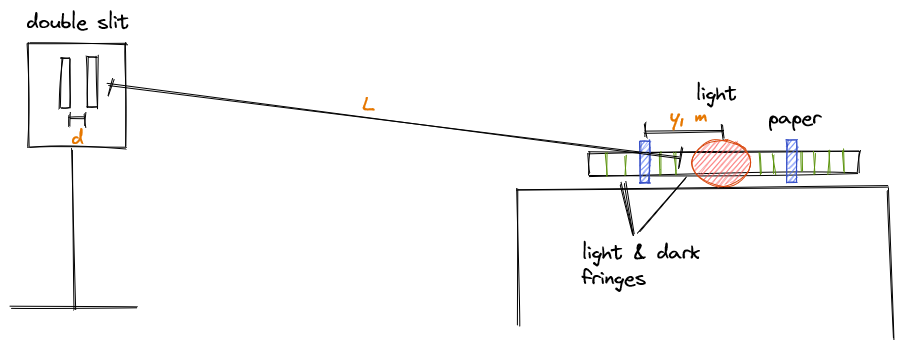
\includegraphics[scale=0.57]{diagram.png}
\caption{Sketch of experiment setup}
\end{figure}

\begin{figure}[H]
\centering
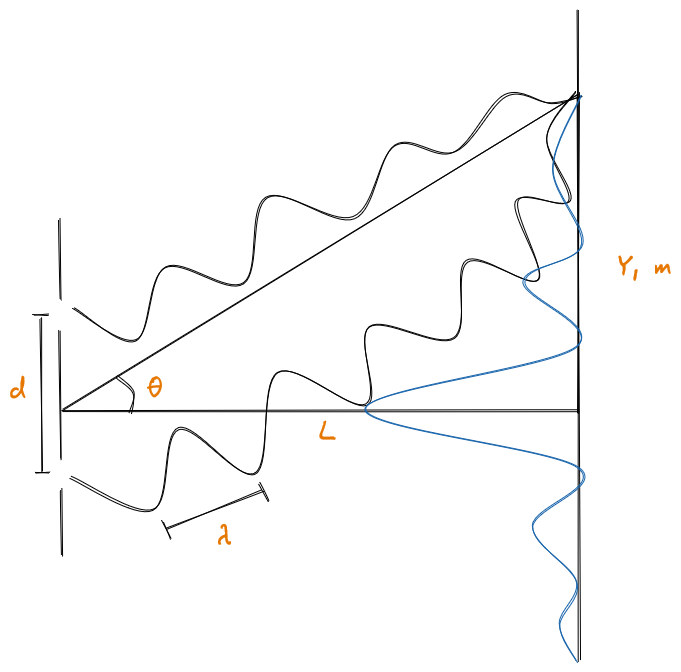
\includegraphics[scale=0.48]{sketch.png}
\caption{Diagram of simplified double-slit diffraction}
\end{figure}

\section{Materials List}

\begin{itemize}
	\item 1 light
	\item 1 double slit with a distance of $0.176\ m$ between both slits
	\item 1 tape measure
	\item 1 ruler
	\item 2 wide and lengthy paper slips
	\item 1 slit stand
\end{itemize}

\section{Procedure}

\begin{enumerate}
	\item Set the slit stand on a flat surface
	\item Fix the slit on the slit stand
	\item Measure 4 meters out from the slit
	\item Place the light at an even level to the stand
	\item Put a meter stick behind the light
	\item Turn on the light
	\item Look through the slits that are $0.176\ m$ apart
	\item From the center of the diffraction pattern, put 1 slip of paper on the closest dark fringe to the left
	\item Repeat the previous step except put the paper slip to the right
	\item Measure the distance between the two slips
	\item Count the number of bright fringes between the two slips
\end{enumerate}

\section{Raw Data Table}

\begin{table}[H]
	\def\arraystretch{1.5}
	\resizebox{\textwidth}{!}{\begin{tabular}{lllll}
			\hline
Distance slit-slit (m) & Distance n-n (m) \(\pm 0.005\) & Order & Distance light-screen (m) \(\pm 0.005\)\\
			\hline
			0.000176               & 0.08             & 3     & 4.14
		\end{tabular}}
\end{table}

\section{Sample Calculations}
\textbf{Calculating the wavelength of the light}
\begin{align*}
	\intertext{We measured a distance of \(0.08 m\) between the two paper slips, but we divide it by 2, since \(y\) only measures the distance from the center to the bright/dark fringe on one side}
	y           & =\frac{0.08\ m}{2}=0.04\ m                       \\
	\intertext{Distance between the slits}
	d           & =0.176\ mm\cdot\frac{1\ m}{1000\ mm}=0.000176\ m \\
	\intertext{Order}
	m           & =3                                               \\
	\intertext{Distance from slit to screen}
	L           & =4.14\ m                                         \\
	\intertext{We have following formula}
	d\sin\theta & =m\lambda                                        \\
	\intertext{Where \(d\) is the distance between the two slits, \(\theta\) is the angle of the diffracted bean of light, \(m\) is the order of interference, and \(theta\) is the wavelenght of light.}
	\intertext{For small angles, }
	\sin\theta  & =\tan\theta=\theta                               \\
	\intertext{So we can replace \(\sin\theta\) with \(\theta\) }
	d\theta     & =m\lambda
\end{align*}
And since \(\tan\theta=\theta\), and \(\tan\) is opposite over adjacent in the following triangle:
\begin{figure}[H]
	\begin{center}
		\begin{tikzpicture}
			\draw (0,0) node[anchor=north]{}
			-- (2,0) node[below]{$L$}
			-- (4,0) node[anchor=north]{}
			-- (4,2) node[right]{$y$}
			-- (4,4) node[anchor=south]{}
			-- cycle;
		\end{tikzpicture}
	\end{center}
\end{figure}
\begin{align*}
	\intertext{We can substitute \(\theta\) with the meaning of \(\tan\)}
	\theta       & =\frac{y}{L}                                                                             \\
	\intertext{This gives us the following}
	d\frac{y}{L} & =m\lambda                                                                                \\
	\intertext{We can divide both sides by \(m\) to get}
	\lambda      & =\frac{dy}{mL}                                                                           \\
	\intertext{We plugin all our values in the table to get}
	\lambda      & =\frac{\left(0.000176\ m\right)\left(0.04\ m\right)}{\left(4.14\ m\right)\left(3\right)} \\
	\Aboxed{     & =5.67\cdot10^{-7}\ m}
\end{align*}

\section{Calculated Data Table}

\begin{table}[H]
	\def\arraystretch{1.5}
	\resizebox{\textwidth}{!}{\begin{tabular}{lllll}
			\hline
Distance slit-slit (m) & Distance n-n (m) \(\pm 0.005\) & Order & Distance light-screen (m) \(\pm 0.005\) & Wavelength of Light (m) \(\pm 0.06\) \\
			\hline
			0.000176               & 0.08             & 3     & 4.14                      & \(5.67 \cdot 10^{-7}\)
		\end{tabular}}
\end{table}

\section{Analysis (Answering the two questions)}


\begin{itemize}
	\item \textbf{What do you observe happening to the diffraction pattern? Describe how the difraction pattern changes as the slit width gets narrower}
	      \subitem As the slit width gets narrower, the distance between the individual dark and light fringes gets wider, and so the diffraction pattern becomes more and more distinguishible.
	\item \textbf{Look through your slitfilm at a white bulb in the clasroom. If you look very carefully at the nodal lines, notice that the bars towards the ends are slightly colored. Why do you think these are colored?}
	      \subitem The bars towards the ends are slightly colored, since the different 'colors' of visible light have different wavelengths. And as the distance from the center increses, closer to the left and right fringes, this difference in wavelength between the different colors becomes visible.
\end{itemize}

\section{Conclusion}

After going through the experiment, I now understand how Young used diffraction by creating two double slits to calculate the wavelength of light. By using basic geometry and what he knew about the wavelength of light, he measured the distance from the screen to the light, the distance between two slits, the order of fringes, as well as the distance from the center to the outer fringe to calculate the wavelength of light.

I also confirmed this by seeing that the distance between the two slits affected the wavelength of light greatly. When I looked through the narrower slit, the distance distance between light and dark fringes got wider. This makes sense, as looking at the derived equation
$$
	\lambda      =\frac{dy}{mL}                                                                           \\
$$
\(d\) and \(y\) seem to have an inversely proportional relationship as they are both on the numerator of the fraciton.

\section{Evaluation of Strengths and Weaknesses}
This experiment had a huge number of flaws. According to literature, the actual wavelength of red light is around $700$ nanometers, which is around \(7\cdot10^{-7}\) meters. This meant that the answer our group measured was off by around $1.33\cdot 10^{-7}$ meters, an error of around \(19\%\)!

The biggest cause of this would probably be the measure of the number of light and dark fringes. Because the lens of the slits might have been touched by fingers and thus become oily, it was extremely difficult to count the warped lines of the dark and light fringes. When we recorded our order of $m=3$, it was more like $m=$ 2--4, with some extra error on where the paper slips were put. This makes sense, as working back from the actual wavelength of \(\lambda=7\cdot10^{-7} m\), and setting $m$ as an unknown like so:

\begin{align*}
7\cdot10^{-7}\ m & =\frac{\left(0.000176\ m\right)\left(0.04\ m\right)}{\left(4.14\ m\right)\left(M\right)}                \\
M                & =\frac{\left(0.000176\ m\right)\left(0.04\ m\right)}{\left(4.14\ m\right)\left(7\cdot10^{-7}\ m\right)} \\
M                & =\boxed{2.43}
\end{align*}

We get the order $M=2.43$, which isn't so far off from what one would expect looking into a very distorted double-slit lens.

\section{Improvements}
The best way to prevent greasy oil stains from distorting lens would just be to not use alens at all. The whole experiment in itself was not actually measuring the diffraction patterns on the screen, as a result of diffraction of the light source, but measuring the patterns on the cornea of the naked eye, and having the light shine on the screen of the eye through the double slit.

Using a finer and steadier light like the lazer pointer through a double slit would make it so that the experiment is actually measuring the real diffracted pattern of the light on a screen, and it would be much easier to read as the person measuring would be able to walk closer and more closely align the paper slips to the diffraction pattern. In other words, everyone would be able to see the diffraction pattern, at whatever distance they choose, rather than the one getting their eyeballs blasted by the diffraction pattern.

Another source of improvement could possibly be to dim the room even further, or move to an area with less light pollution, as sometimes with many experiments going on in close proximity, the lights clashed and it was harder to make out the outlines of the dark and light fringes and thus was harder to determine the number and order of the fringes.
\end{document}
